

%\section{Graph Decomposition \del{based problem formulation}}
\section{\rev{Graph Decomposition}}
\label{lab:Graphdecompositionbasedproblemformulation}
\rev{In order to ensure survivable virtual network embedding, backup resources need to be added
to guarantee that the remaining physical resource plus the backup resources can still support a feasible mapping when any a physical node fails.} To facilitate \rev{the finding of  feasible mapping upon node failure, we first decompose} the virtual network and physical network into star-based local components. Based on which, a novel   bipartite graph is proposed and the problem of survivable virtual network embedding with low backup cost is formulated as a virtual star assignment problem based on the well defined bipartite graph.


%with the edge weight  intelligently  denoting the backup resource cost to map virtual network components to the physical components. Based on the graph, the minimum backup cost Survivable virtual network embedding is modeled as a constrained multiple  knapsack problem which is proved to be NP-hard problem.
\subsection{Star based graph decomposition}
To capture  the relationship \rev{between the virtual and physical nodes} with its adjacent \note{what do you mean "with its adjacent"?} thus facilitate the problem formulation, we propose a novel algorithm to decompose the virtual network and physical network into star based local structures.


Specially, \rev{a} virtual network is decomposed into virtual local stars with each star associated with a virtual node. Given a virtual node $v_i$, the corresponding virtual local star is defined as \rev{an attributed single-level tree rooted at $v_i$:}

\begin{equation}
VS(i)=(v_i, \phi(v_i), d_i, f_i, D_i, N(i))
\label{eq:virtualstar}
\end{equation}
where $N(i)$ is the neighbor node set of $v_i$ in the virtual network and \rev{the bandwidth demand set} ${D_i} = \left\{ {{d_{ij}}|{v_j} \in {N(i)}} \right\}$. \rev{The} virtual Star VS($v_i$) includes the node mapping information $\phi(v_i)$. \rev{To minimize the backup resources, reusing} the mapping before node failure may be a good choice to reduce the additional resources and make the system remain stable. In the virtual star structure, \rev{there are} edges  between the root node and its neighbor nodes, but no edge exists \rev{between any two} neighbor nodes.

The physical network is decomposed into physical local stars, \rev{each is} associates with a physical node. Given a physical node $s_j$, the corresponding physical local star is defined as \rev{an attributed single-level tree rooted at $s_j$}

\begin{equation}
PS(j)=(s_j, \phi^{-1}( s_j), c_j, F(j), \phi(N(\phi^{-1}( s_j))), \xi(s_j))
\label{eq:physicalstar}
\end{equation}
where $\phi^{-1}( s_j) $ are all virtual nodes that are mapped to the physical node $s_j$, $N(\phi^{-1}( s_j))$ is the neighbor nodes of the virtual nodes in $\phi^{-1}( s_j)$, $\phi(N(\phi^{-1}( s_j)))$ are the physical nodes that hold these neighbors, $c_j$ is the node capacity, $F(j)$ is the virtual functions supported by $s_j$,  $\xi(s_j)$ is a one-bit single with its value being 0 or 1 to indicate whether this physical node has \rev{set up} the virtual machine or not. Similar to virtual star, in the physical star structure, edges exist between the root node and its neighbor nodes \rev{but do not exist between any two neighbor nodes.}

After network decomposition, a virtual network \rev{consisting} of $n=|V|$ virtual nodes will be decomposed into $n=|V|$ virtual stars. A physical network \rev{with} $m=|S|$ physical nodes will be decomposed into $m$ physical stars. Virtual star and physical star defined in (\ref{eq:virtualstar}) and (\ref{eq:physicalstar})  well capture the local structures hidden in the virtual network and the physical network to preserve the relationship of \rev{a node with its adjacent nodes.}

.
\subsection{Bipartite graph}
Based on the virtual local stars and physical local stars, \note{why physical is also called virtual?}  the virtual network and physical network can be decomposed into multiple components.
We build a bipartite graph $G=\{VS,PS,E\}$ to present the relationship between the virtual network and physical network. In the bipartite graph,
$VS$ and $PS$ are the vertex sets  representing the set of virtual stars and the set of physical stars, respectively. If $VS(i)$'s virtual function $f_i$ can be executed by a physical node $s_j$ with ${f_i} \in {F_j}$, an edge $e(i,j)$ is added to the edge set $E$ to connect $VS(i)$ and $PS(j)$.

Our goal is to minimize the backup resource to provide survivable service. To achieve the goal, \rev{for an} edge $e(i,j)$ in the bipartite graph, we define the edge weight $w(i,j)$  as the backup resource cost to map the virtual star $VS(v_i)$ to the physical star $PS(s_j)$ when  node failure happens. According to whether the virtual node $v_i$ is mapped to the physical node $s_j$ before node fails, we define the edge weight $w(i,j)$ in two different cases.

%\begin{equation}
%\footnotesize
%Vactive(v_i) = \left\{ {\begin{array}{*{20}{c}}
%   { 1 } & {\phi(v_i)\ is failed}  \\
%   {0 } & {v_i\ is\ active}  \\
%\end{array}} \right.
%\label{eq:Vactive}
%\end{equation}

\begin{equation}
\footnotesize
Pactive(s_j) = \left\{ {\begin{array}{*{20}{c}}
   { 1 } & {\phi(s_j)\ is failed}  \\
   {0 } & {s_j\ is\ active}  \\
\end{array}} \right.
\label{eq:Vactive}
\end{equation}


\begin{equation}
\footnotesize
w(i,j) = \left\{ {\begin{array}{*{20}{c}}
   { \alpha \sum\limits_{v_k\in N(i)} {{d_{ik}}}*{Pactive(\phi(v_k))} } & {{v_i} \in {\phi ^{ - 1}}({s_j}),Pactive(s_j)=0}  \\
   {\delta+{M_m}+\lambda {d_i}+\alpha \sum\limits_{v_k \in N(i)} {{d_{ik}}}    } & {{v_i} \notin {\phi ^{ - 1}}({s_j}),Pactive(s_j)=0}  \\
   {\infty} & {Pactive(s_j)=1}  \\
\end{array}} \right.
\label{eq:edge weight}
\end{equation}
In Eq.(\ref{eq:edge weight}), $\delta$ is defined as follows.
\begin{equation}
\delta  = \left\{ {\begin{array}{*{20}{c}}
   {{C_s}} & {\xi(s_j) = 0}  \\
   0 & {\xi(s_j) = 1}  \\
\end{array}} \right.
\end{equation}

\note{What is $\xi$?}
In the first case (${v_i} \in {\phi ^{ - 1}}({s_j})$) in Eq.(\ref{eq:edge weight}), as the virtual node $v_i$ is mapped to the physical node $s_j$ before node fails, the node capacity demand is satisfied already, thus only the bandwidth backup cost is counted when \rev{mapping} the virtual star ($v_i$) to the physical star ($s_j$). For each neighbor $v_k \in N(i)$ , if  the physical node that holds virtual node $v_k$ fails with ${\phi ({v_k}) \notin \phi (N({\phi ^{ - 1}}({s_j})))}$, new path with bandwidth $d_{ik}$ should be added as the backup resource. Therefore, in this case, the backup cost only includes \rev{the} bandwidth cost and is expressed as $ { \alpha \sum\limits_{\phi ({v_k}) \notin \phi (N({\phi ^{ - 1}}({s_j})))} {{d_{ik}}} }$ where $\alpha$ is the unit bandwidth weight. \note{I don't understand why do you set up the link weight, and why the link weight is set as the demand when a neighbor fails. I thought link weight is put in advance to guide the backup path selection later. Also, which node failure are you considering vi or vk? In addition, in the subscript of the second equation, you put $k$ not $v_k$}
%$k\in N(i}$ not $v_k \in N(i)$.}

In the second case (${v_i} \notin {\phi ^{ - 1}}({s_j})$), as the virtual node $v_i$ is not mapped to the physical node $s_j$ before node fails,  \rev{it needs to be migrated to the} physical node $s_j$. Therefore, the edge weight $w(i,j)$ includes \rev{the cost to take node's computational capacity}  ($\lambda {c_i}$ where $\lambda$ is the
unit capacity cost), \rev{the cost of path bandwidth} ($\alpha \sum\limits_{k \in N(i)} {{d_{ik}}}$), and \rev{the cost} (${M_m}$) to migrate a virtual node from a physical node to another physical node when physical nodes fail. \note{I don't know which physical node you refer to as the failure node.}  Moreover, if the backup physical node $s_j$ does not  hold any virtual node before, migrating a virtual node to this physical node also introduces a \text{virtual machine booting  cost}, denoted as $C_s$.

\note{I don't follow figure 3. in (a), you have only four physical nodes. Why in (b) PS you have more physcial nodes? For each physical stars, you are not showing physical connection but also virtual nodes?}

Fig.\ref{fig:StarRepresentation} shows \rev{an example of such a bipartite graph when the} physical node $s_1$ fails. The edge weight of this   bipartite graph \rev{is} shown in Fig.\ref{fig:StarRepresentation}(c).
\begin{figure}
\centering
% Requires \usepackage{graphicx}
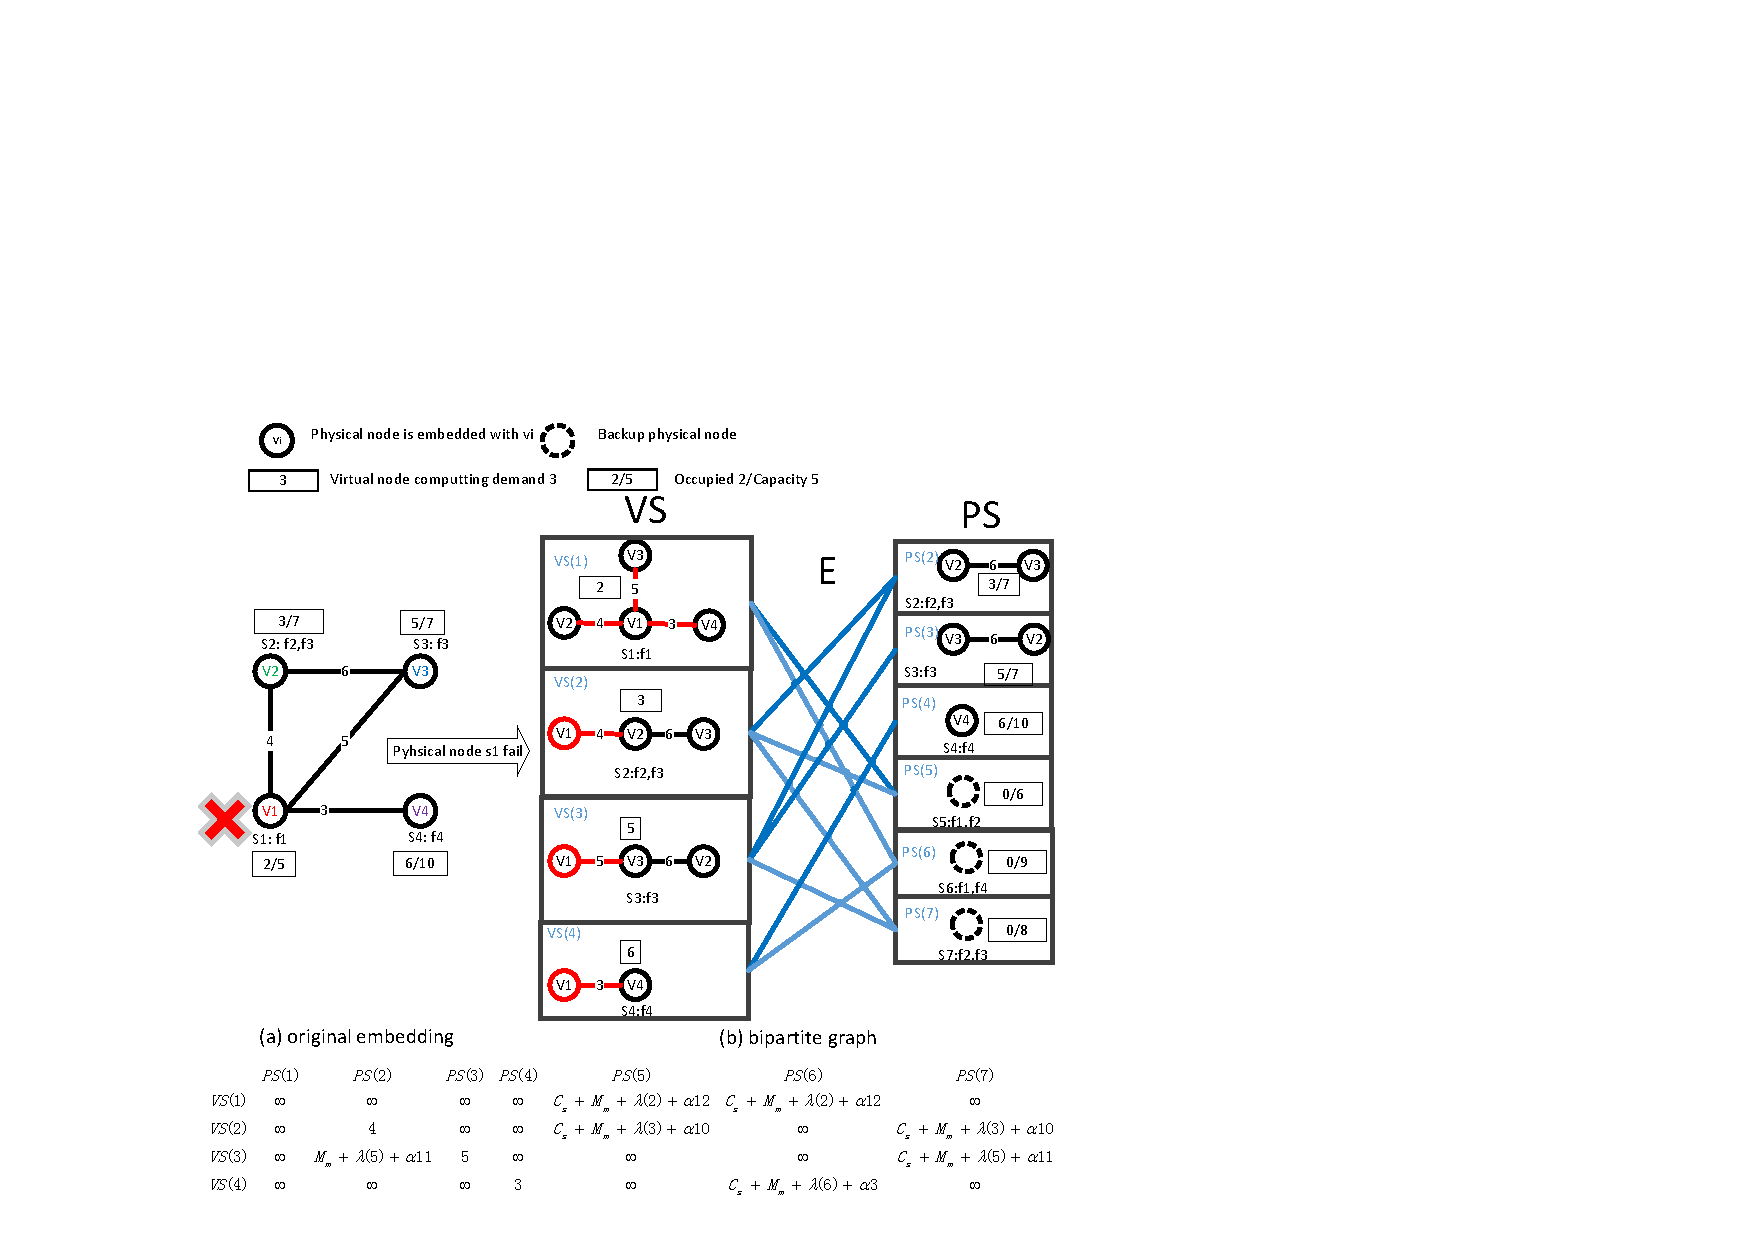
\includegraphics[width=3.7in]{Fig/StarRepresentation}\\
  \caption{Bipartite graph when physical node $s_1$ fails}\label{fig:StarRepresentation}
\end{figure}

%\begin{equation}
%\tiny{
%\[\begin{array}{*{20}{c}}
%{}&{PS(1)}&{PS(2)}&{PS(3)}&{PS(4)}&{PS(5)}&{PS(6)}&{PS(7)}\\
%{VS(1)}&\infty &\infty &\infty &\infty &{{C_s} + {M_m} + 2\lambda  + 12\alpha }&{{C_s} + {M_m} + 2\lambda  + 12\alpha }&\infty \\
%{VS(2)}&\infty &4\alpha&\infty &\infty &{{C_s} + {M_m} + 3\lambda  + 10\alpha }&\infty &{{C_s} + {M_m} + \lambda 3 + 10\alpha }\\
%{VS(3)}&\infty &{{M_m} + 5\lambda  + 11\alpha }&5\alpha&\infty &\infty &\infty &{{C_s} + {M_m} + 5\lambda  + 11\alpha }\\
%{VS(4)}&\infty &\infty &\infty &3\alpha&\infty &{{C_s} + {M_m} + 6\lambda  + 3\alpha }&\infty
%\end{array}\]
%}
%\label{lab:Node1FaliureAlignmentMatrixNew}
%\end{equation}


%\begin{equation*}
%\tiny{
% {\begin{array}{*{20}{c}}
%&{L_{V_1}}&L_{V_2}&L_{V_3}&L_{V_4}\\
%R_{S_{1}}&\infty&\infty&\infty&\infty\\
%R_{S_{2}}&\infty&\fbox{4}&M_{m}+(5)+11&\infty\\
%R_{S_{3}}&\infty&\infty&\fbox{5}&\infty\\
%R_{S_{4}}&\infty&\infty&\infty&\fbox{3}\\
%R_{S_{5}}&\fbox{$C_{s}+M_{m}$+(2)+12}&C_{s}+M_{m}+(3)+10&\infty&\infty\\
%R_{S_{6}}&C_{s}+M_{m}+(2)+12&\infty&\infty&C_{s}+M_{m}+(6)+3\\
%R_{S_{7}}&\infty&C_{s}+M_{m}+(3)+10&C_{s}+M_{m}+(5)+11&\infty\\
%\end{array}}
%}
%\label{lab:Node1FaliureAlignmentMatrixNew}
%\end{equation*}





For the virtual node $v_i$, if its virtual function can not be executed in physical node $s_j$
with \rev{$f(i) \notin F(j)$,} \note{I changed the previous equation, please double check.} no edge is connected \rev{between} $VS(v_i)$  and $PS(s_j)$. To facilitate \rev{the} problem formulation, we \rev{set the edge weight to} $\infty $. For example, as $v_1$'s virtual \rev{function $f_1$ can not be executed in physical node $s_2$, no edge is added to connect $VS(v_1)$ and $PS(s_2)$, and we set $w(1,2)=\infty$.}

For $VS(v_2)$, \rev{$v_2$ is originally held by $s_2$. When the} physical node $s_1$ (which holds $v_1$ originally) fails, the virtual link $e_{12}$ fails \rev{to map to} \note{Here it has passive meaning without need of explicitly put as be mapped.} the physical network. We should find a new path \rev{that connects   $\phi(v_2)$ with $\phi(v_1)$ and satisfies the} bandwidth demand  $d_{12}=4$. Therefore, the edge weight connecting $VS(v_2)$ and $PS(s_2)$ is $4\alpha$. \note{TO be frank, I don't follow your two cases in equation 3.}

When node $s_1$ fails, it directly impacts the virtual node $v_1$. As $s_5$ can execute \rev{the} virtual function $f_1$, we can add an edge to  connect $VS(v_1)$ and $PS(s_5)$. However, as $s_5$ \rev{does not have the virtual machine set up before, it also introduces the virtual machine} startup cost $C_s$.  Therefore, the edge weight is $C_s$ (startup cost)+ $M_m$ (migrating cost)+ $3\lambda $ (node computation cost)+ $10\alpha$ (link bandwidth cost). \note{Please check. You mentioned a a wrong matrix mapping in (c). You are talking about connection between V2 and PS2.}

\subsection{Problem formulation}
To provide \rev{a} survivable service, each virtual star (both the root virtual node and \rev{its virtual links connecting to the} adjacent nodes) should be mapped to a physical star. In Eq(\ref{eq:indication}), we use \rev{the binary variable} $M_{ij}$ to denote whether  the $i$-th virtual star is mapped to the $j$-th physical star.
\begin{equation}
{M_{ij}} = \left\{ {\begin{array}{*{20}{c}}
   1 & {map \ v_i \  to  \ s_j}  \\
   0 & {otherwise}  \\
\end{array}} \right.
\label{eq:indication}
\end{equation}
In our bipartite graph, the edge weight is defined as the backup cost to map the corresponding virtual star to the physical star when a physical node fails. \rev{To minimize} the backup resource cost, the survivable virtual network embedding problem can be defined as:
\begin{equation}
\begin{array}{*{20}{c}}
   {\mathop {\min }\limits_{{M_{ij}}} } & {\sum\limits_{i = 1}^n {\sum\limits_{j = 1}^m {{M_{ij}}{w_{ij}}} } }  \\
   {s.t.,} & {\sum\limits_{i = 1}^n {{d_i}{M_{ij}}}  \le {c_j}}  \\
   {} & {\sum\limits_{j = 1}^m {{M_{ij}}}  = 1}  \\
   {} & {{M_{ij}} = \{ 0,1\} }  \\
\end{array}
\label{eq:problem formulation}
\end{equation}
where ${\sum\limits_{i = 1}^n {\sum\limits_{j = 1}^m {{M_{ij}}{w_{ij}}} } }$ denotes the total backup resource  cost to map all \del{the} virtual stars to physical stars when physical nodes fails.  In Eq(\ref{eq:problem formulation}), ${\sum\limits_{i = 1}^n {{d_i}{M_{ij}}}  \le {c_j}}$ is \rev{the capacity constraint of the physical node. That is,} even though multiple virtual nodes are allowed to be mapped to a physical node, the total capacity demand should not \rev{exceed} the capacity of the physical node. ${\sum\limits_{j = 1}^m {{M_{ij}}}  = 1}$ indicates that one virtual star can be mapped to only one physical star.

Obviously, the problem defined in (\ref{eq:problem formulation}) is a binary ILP assignment problem, which is general an NP-complete problem according to Karp's 21 NP-complete problems\cite{karp1975computational}. %In following  Theorem 1, we validate the theorem.

\textbf{Theorem 1} Problem defined in (\ref{eq:problem formulation}) is an NP-complete problem.
\begin{proof}
If  there is only one physical node with $m=1$, our survivable virtual network embedding problem can be  \rev{degenerated} into \rev{the} single knapsack problem, which is NP-complete \del{ problem}. In practice, $m$ is usually larger than 1, \rev{so a} single knapsack problem is \rev{a} subproblem of survivable virtual network embedding problem. \note{You should separate sentences.} \rev{Given} a feasible solution is easily verified in polynomial time, according to the reducibility theorem\cite{wood1987theory} in computer complexity field, it is easy to conclude that our defined in (\ref{eq:problem formulation}) is also NP-complete.
\end{proof}

\section{Dynamic programming based algorithm}
\label{lab:DynamicProgrammingEquation}

Although solving the ILP formulation will result in the optimal solution, its exponential time complexity makes \rev{it impractical to apply for embedding a virtual network into} a large  physical network. In this section, we propose a dynamic programming based algorithm that has only a polynomial time complexity \rev{for the application in} practical network systems.


%To describe our  dynamic programming based virtual node mapping algorithm,
We define  $dp[i][{x_1}][{x_2}] \ldots [{x_m}]$ to denote the best virtual star placement with the minimum backup resource cost to have the first $i$ ($0 \le i \le n=|V| $) virtual stars placed \rev{on} the $m=|S|$ physical stars \rev{whose root nodes have the physical capacity limits $ x_1$, $ x_2$, $\ldots$, $x_m$.}

The $i$-th virtual star has the option to  be placed onto any one of the physical stars that are alive. Let $\theta (i,j)$ denote \rev{the cost of} the backup resources to place the $i$-th virtual node \del{star} to the $j$-th physical node after the first $i-1$ virtual nodes are best placed. $\theta (i,j)$ is expressed as follows.
\begin{equation}
\footnotesize
\theta (i,j) = \left\{ {\begin{array}{*{20}{c}}
{dp[i - 1][x_1][{x_2}] \ldots [{x_j} - {d_i}] \ldots [{x_m}] + {w_{ij}}}\\
\infty
\end{array}} \right.\begin{array}{*{20}{c}}
{({x_j} \ge {d_i},{f_i} \in {F_j})}\\
{otherwise}
\end{array}
\label{eq:place i to j}
\end{equation}
In (\ref{eq:place i to j}), if the capacity  limit of the  physical node $x_j$ is larger than the capacity demand $d_i$ and the virtual function $f_i$ can be executed \rev{by} the physical node ${f_i} \in {F_j}$,  $\theta (i,j)$ is the \rev{summation} of   the cost under \rev{the} best virtual star placement \rev{where the first $i-1$ ($0 < i \le n $) virtual stars are placed to} the $m$ physical stars  (i.e., $dp[i-1][{x_1} - {d_i}][{x_2}] \ldots [{x_m}]$) and the cost \rev{to map} the virtual star ($v_i$) to \rev{the} physical star ($s_1$) (i.e., $w_{i1}$ ). \note{You put $w_{ij}$. Overall, it is very confusing what you are doing.}


\note{Why do you have the ${x_j} - {d_i}$ in the equation and ${x_1} - {d_i}$ also? I thought you only want to put the capacity limit, and why putting the difference and also putting two different values? A node not only serves this request but may be also other requests. You simply use the capacity to deduct the demand of this request does not appear to be reasonable.}

Based on $\theta (i,j)$, $dp[i][{x_1}][{x_2}] \ldots [{x_m}]$ can be calculated through the following dynamic programming function.
\begin{equation}
dp[i][{x_1}][{x_2}] \ldots [{x_m}] = min\{\theta (i,1),\theta (i,2),\ldots,\theta (i,j),\ldots,\theta (i,m)\}
\label{eq:update function}
\end{equation}


\begin{algorithm}
\label{alg:DPAlg}
\caption{Based Dynamic Programming Virtual Node Mapping  Algorithm}
\begin{algorithmic}[1]
\REQUIRE {$dp[i][{x_1}][{x_2}] \ldots [{x_m}]=0(1\leq i \leq n, 0\leq x_1\leq c_1, 0\leq x_2\leq c_2,\ldots, 0\leq x_m\leq c_m)$ is firstly assigned as infinity $\infty$, $dp[0][{x_1}][{x_2}] \ldots [{x_m}]=0(0\leq x_1\leq c_1, 0\leq x_2\leq c_2,\ldots, 0\leq x_m\leq c_m)$, m is the number of physical nodes. $M[{x_1}][{x_2}] \ldots [{x_m}]=\textbf{0}_{n\times m}$ is \rev{the matrix identifying the} virtual node mapping.}
\ENSURE {obtaining the lowest \rev{overall cost with the} virtual node mapping matrix \rev{when the up-bound  capacity of physical nodes} is $c_1,c_2,\ldots,c_m$, respectively.}
\FORALL{$i$ such that $1\leq i\leq n$ }
\FORALL{$x_1,x_2,\ldots,x_m$ such that $ c_1\geq x_1\geq d_i$, $c_2\geq x_2\geq d_i$,$c_3\geq x_3\geq d_i$,$c_m\geq x_m\geq d_i$}

\STATE {$dp[i][{x_1}][{x_2}] \ldots [{x_m}] = min\{\theta (i,1),\theta (i,2),\ldots,\theta (i,j),\ldots,\theta (i,m)\}$}

\STATE{$j' = \mathop {\arg \min }\limits_j \{\theta (i,1),\theta (i,2),\ldots,\theta (i,j),\ldots,\theta (i,m)\}$, }.
\STATE{$M[{x_1}][{x_2}] \ldots [{x_m}]=M[{x_1}][{x_2}] \ldots[x_{j'}-d_i]\ldots [{x_m}]$}
\STATE{$M[{x_1}][{x_2}] \ldots [{x_m}]_{ij'}=1$}
\ENDFOR
\ENDFOR
\RETURN $dp[i][{c_1}][{c_2}] \ldots [{c_m}]$ and $M[{c_1}][{c_2}] \ldots [{c_m}]$
\end{algorithmic}
\end{algorithm}

%\left[ {\begin{array}{*{20}{c}}
%0&0&0&0&0&0&0\\
%0&0&0&0&0&0&0\\
%0&0&0&0&0&0&0\\
%0&0&0&0&0&0&0
%\end{array}} \right]
The pseudo-code of the dynamic programming based algorithm is shown in Alg.\ref{alg:DPAlg}.
We further use an example in Fig.\ref{fig:DPIllustration} to illustrate the algorithm.


\begin{figure}
\centering
% Requires \usepackage{graphicx}
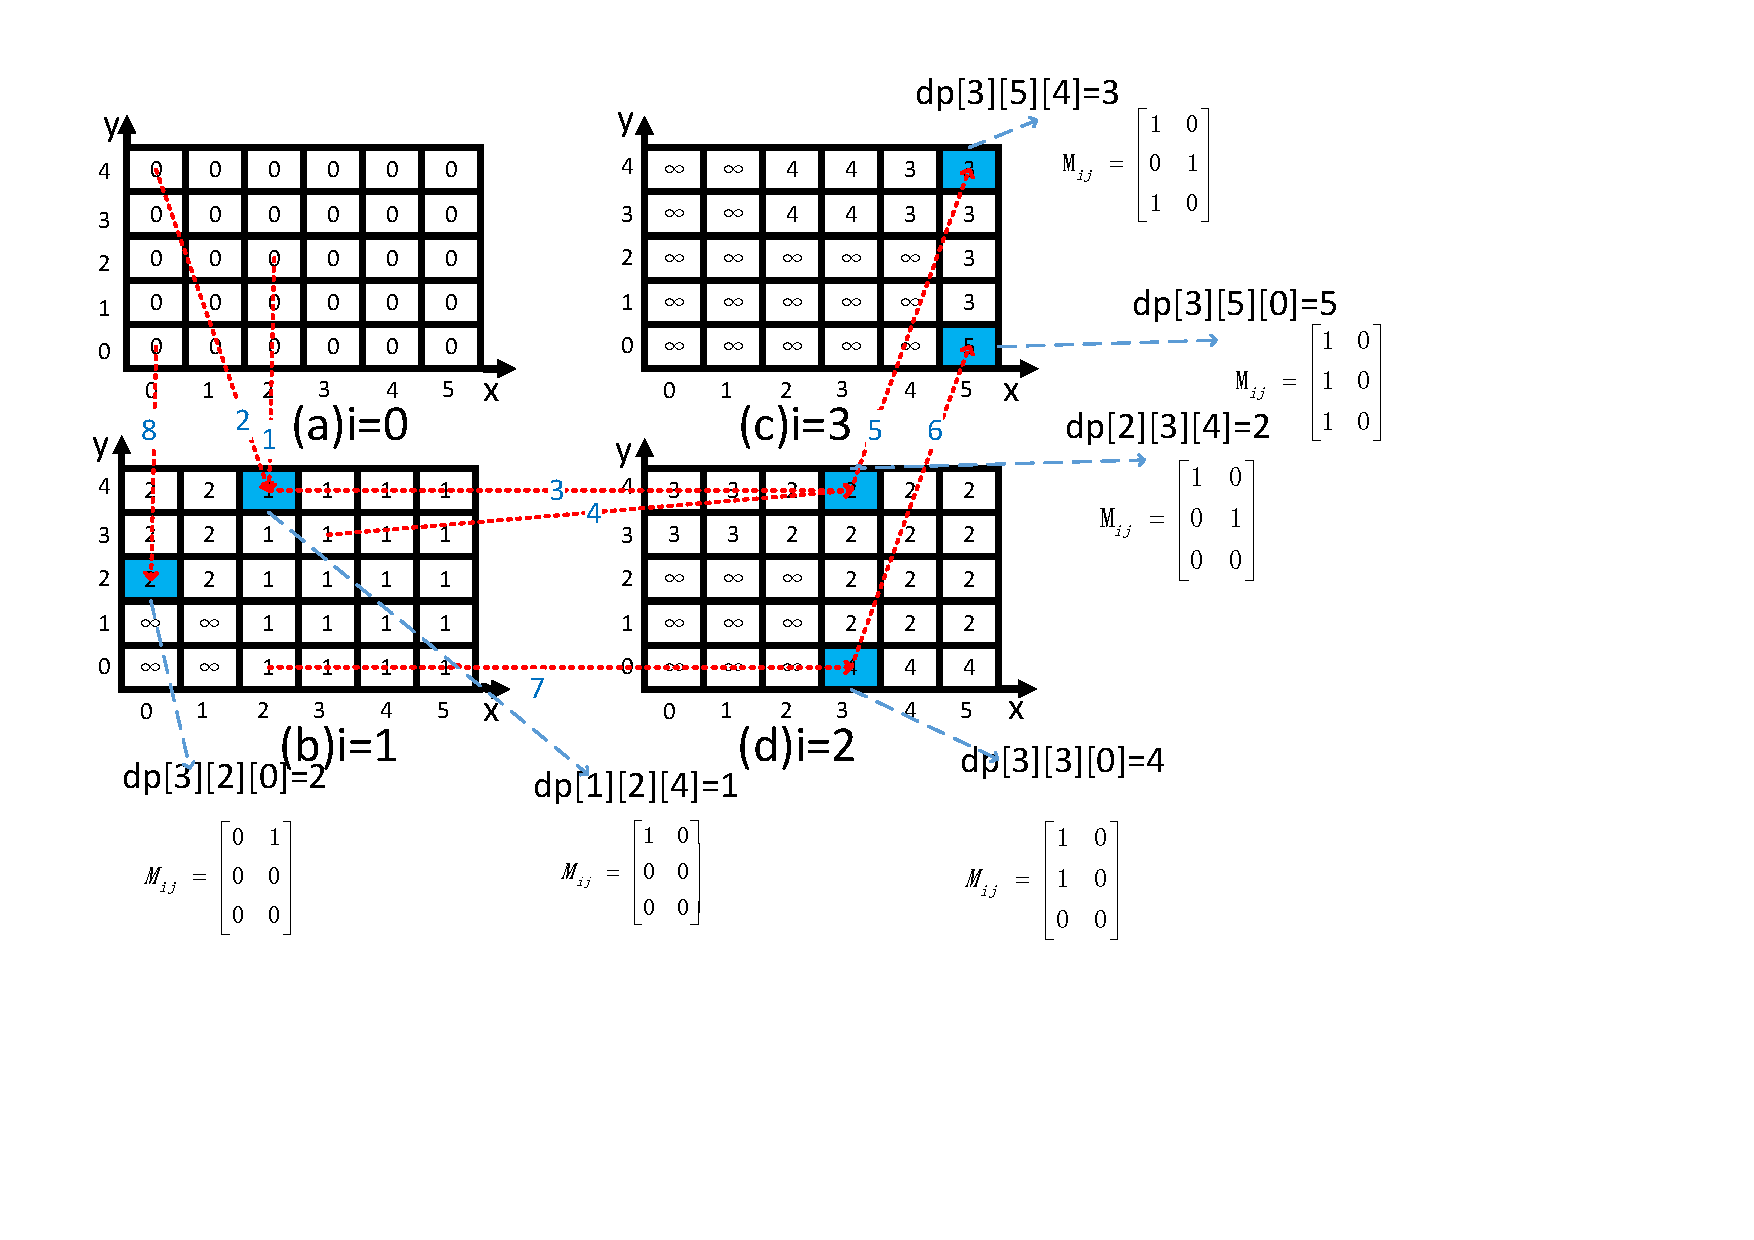
\includegraphics[width=4in]{Fig/DPIllustration}\\
  \caption{An example to illustrate the dynamic programming based algorithm.} %Three virtual node, the first virtual node could be placed to first and second physical node,  the second virtual node could be placed to first and second physical node,  the third virtual node could only be placed to first physical node.  The  node computation capacity of first physical node is 5, the node computation capacity of second physical node is 4. $w_{ij}$=[1,2;3,1;1,$\infty$].}
  \label{fig:DPIllustration}
\end{figure}



 \rev{In this example, three virtual stars} need to be placed \rev{onto} two available physical stars to achieve the minimum backup  cost. The available capacity \rev{of} physical nodes are $c_1=5$ and $c_2=4$, respectively. The capacity demands of these three virtual stars are $d_1=2$, $d_2=1$, and $d_3=2$. The virtual functions required to be executed \rev{by} these virtual stars are $f(1)=f_1$, $f(2)=f_1$, $f(3)=f_2$. The functions supported by \rev{the} two physical nodes are $F(1)=\{f_1,f_2\}$ and $F(2)=\{f_1\}$.

In Fig.\ref{fig:DPIllustration}, $x$ and $y$ \rev{axes} denote the capacity \rev{limits of physical stars} $s_1$ and $s_2$, respectively. \note{But you have 5 items on the X axix and 4 items on the Y axis.} The  \rev{weights of edges} connecting virtual stars to physical stars are $w_{11}=1$, $w_{12}=2$, $w_{21}=3$, $w_{22}=1$, $w_{31}=1$, $w_{32}=\infty$, respectively.


Initially, in Fig.\ref{fig:DPIllustration}(a), as no virtual star is placed to any physical stars, the backup cost under all the capacity limit cases ($x_1=0, 1, 2, 3, 4$ and $x_2=0, 1, 2, 3, 4, 5$) \note{Why do you have so many capacity limits?} are all 0. Specially, even though capacity limits are set 4 and 5, dp[0][4][5]=0. \note{Don't know what you want to say in this sentence.}

In Fig.\ref{fig:DPIllustration}(b), when place the first virtual node $v_1$ with capacity demand $d_1=2$ to these two physical nodes, as $f_1$ can be executed in both physical nodes,  we have
\begin{equation}
dp[1][{x_1}][{x_2}] = \min \{\theta (1,1),\theta (1,2)\}
\end{equation}
Specially, if the capacity limit of these two physical nodes are $x_1$=2 and $x_2$=0, we have $dp[1][2][0]= dp[0][0][0]+w_{11}=2$. If the capacity limit of these two physical nodes are $x_1$=2 and $x_2$=4, we have $\theta (1,1)=dp[0][0][2]+w_{11}$ and $\theta (1,2)=\infty$ and thus $dp[1][2][4]=min\{ dp[0][0][4]+w_{11}), dp[0][2][2]+w_{12} \}=1$.

Similarly, when place the second virtual node with capacity demand $d_2=1$ to these two physical nodes, the cost results under all capacity limits is shown in Fig.\ref{fig:DPIllustration}(d). As $f_2$ can be executed in both physical nodes, thus $v_2$ can be placed into both physical nodes, we have
\begin{equation}
dp[2][{x_1}][{x_2}] = \min \{\theta (2,1),\theta (2,2)\}
\end{equation}
Specially, if the capacity limit of these two physical nodes are $x_1$=3 and $x_2$=4, we have $dp[2][3][4]=min\{dp[1][2][4]+w(2,1), dp[1][3][3]+w(2,2)\}=2$. If the capacity limit of these two physical nodes are $x_1$=3 and $x_2$=0, we have $dp[2][3][0]=dp[1][2][0]+w(2,1)=4$.

Fig.\ref{fig:DPIllustration}(d) shows the minimum resource cost result  when  place the third virtual node with capacity demand $d_3=2$ to these two physical nodes. As $f_3$ can only be executed in physical node $s_1$, we have $\theta (3,2)=\infty$. Specially, if the capacity limit of these two physical nodes are $x_1$=5 and $x_2$=0, we have $dp[3][5][0]=dp[2][3][0]+w(3,1)=4$. As the node capability of these two physical nodes are 5 and 4, respectively, we have $dp[3][5][4]=dp[2][3][4]+w(3,1)=3$, as indicted in Fig.\ref{fig:DPIllustration}(d), the best placement is achieved at dp[3][5][4]=3 with the node mappping $\phi{v_1}= s_1, \phi{v_2}=s_2, \phi{v_3}=s_1$. Therefore, virtual node mapping matrix is
$M_{3 \times 2}=\left[ {\begin{array}{*{20}{c}}
1&0\\
0&1\\
1&0
\end{array}} \right]$.

For the example in Fig.\ref{fig:StarRepresentation}, if the mapping matrix is $M_{ij}=\left[ {\begin{array}{*{20}{c}}
0&0&0&0&1&0&0\\
1&0&0&0&0&0&0\\
0&1&0&0&0&0&0\\
0&0&1&0&0&0&0
\end{array}} \right]$, we can obtain the survivable virtual network embedding is shown in Fig.\ref{fig:Node1Failure}(b).


%For example, as shown in Fig.\ref{fig:StarRepresentation} and Equ.(\ref{lab:Node1FaliureAlignmentMatrixNew}), the optimal $M_{ij}=\left[ {\begin{array}{*{20}{c}}
%0&0&0&0&1&0&0\\
%1&0&0&0&0&0&0\\
%0&1&0&0&0&0&0\\
%0&0&1&0&0&0&0
%\end{array}} \right]$.


\begin{figure}
\centering
% Requires \usepackage{graphicx}
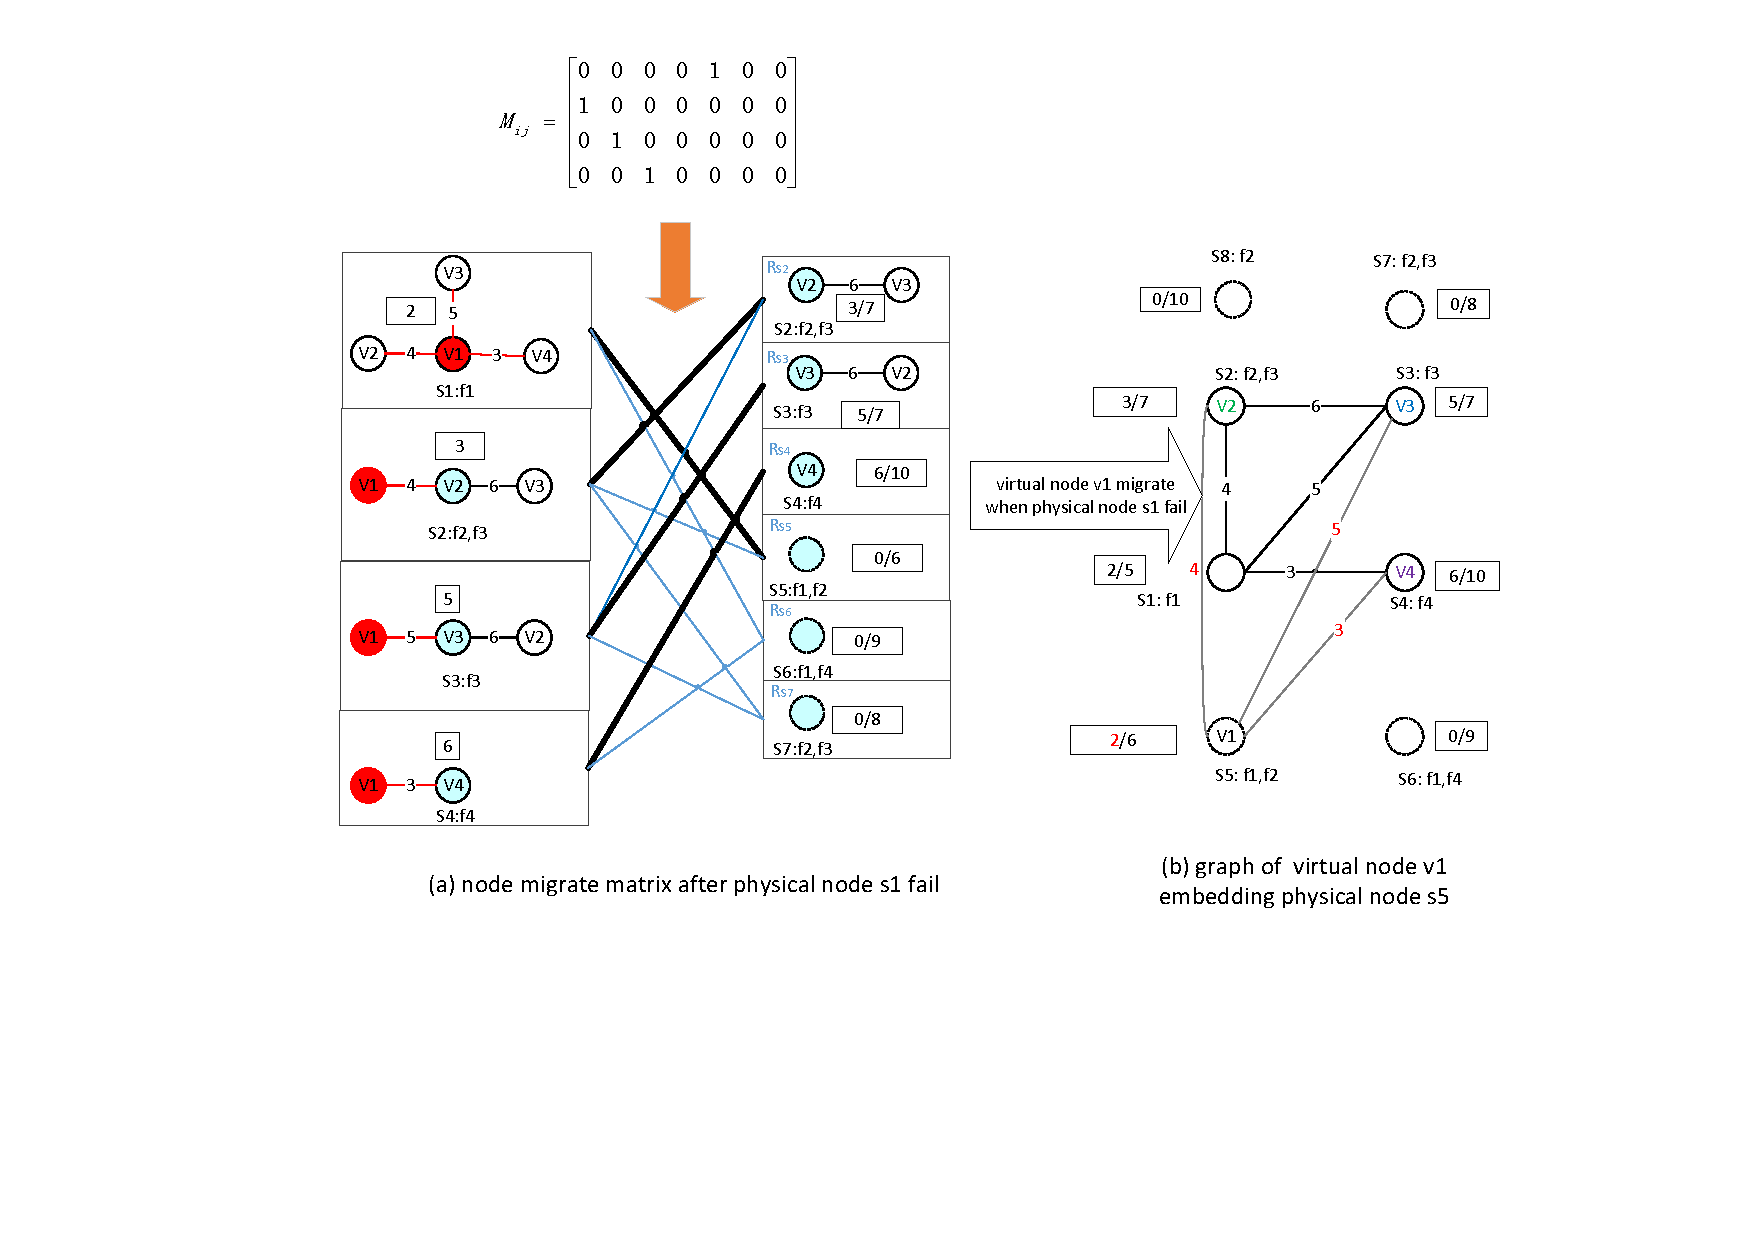
\includegraphics[width=4in]{Fig/Node1Failure}\\
  \caption{The survivable virtual network embedding after physical node $s_1$ fails}\label{fig:Node1Failure}
\end{figure}










Given the VN request $G (V,E)$ with $n = \left| V \right|$ virtual nodes and the physical network  $G (S,L)$ with $m = \left| S \right|$ physical nodes,  our dynamic programming based algorithm finds the best mapping between virtual stars and physical stars by testing each virtual star's placement. Each testing is called one round. There are $\prod_{i=1}^{m}C^i$ dynamic programming functions in every round with the time complexity of calculating each dynamic programming function is $O(m)$ according to Eq.\ref{eq:update function}. Therefore, the overall time complexity of the dynamic programming method is $n*\prod_{i=1}^{m}C^i*O(m)=O(n*m*\prod_{i=1}^{m}C^i)$. Additionally, for recording every round's virtual node's placement, the overall space complexity is $O[(n+1)*\prod_{i=1}^{m}C^i]$. However, it could be optimized to $O[\prod_{i=1}^{m}C^i]$, because when updating every round values of the dynamic programming functions, only one previous round's  values of the dynamic programming functions are used and  all the other previous rounds' values of  dynamic programming functions  are no longer to be used and stored.




